% # 3.1 共享数据的问题

涉及到共享数据时,问题就是因为共享数据的修改所导致。如果共享数据只读,那么不会影响到数据,更不会对数据进行修改,所有线程都会获得同样的数据。但当一个或多个线程要修改共享数据时,就会产生很多麻烦。这种情况下,需要小心谨慎,才能确保所有线程都正常工作。

不变量(invariants)的概念对开发者们编写的程序会有一定的帮助——对于特殊结构体的描述,比如:“变量包含列表中的项数”。更新通常会破坏不变量,特别是复杂的数据结构。

双链表中每个节点都有一个指针指向列表中下一个节点,还有一个指针指向前一个节点。其中不变量就是节点A中指向“下一个”节点B的指针,还有前向指针。为了从列表中删除一个节点,其两边节点的指针都需要更新。当其中一边更新完成时,就破坏了不变量,直到另一边也完成更新。在两边都完成更新后,不变量就稳定了。

从一个列表中删除一个节点的步骤如下(如图3.1)

   a. 找到要删除的节点N

   b. 更新前一个节点指向N的指针,让这个指针指向N的下一个节点

   c. 更新后一个节点指向N的指针,让这个指正指向N的前一个节点

   d. 删除节点N

\begin{center}
    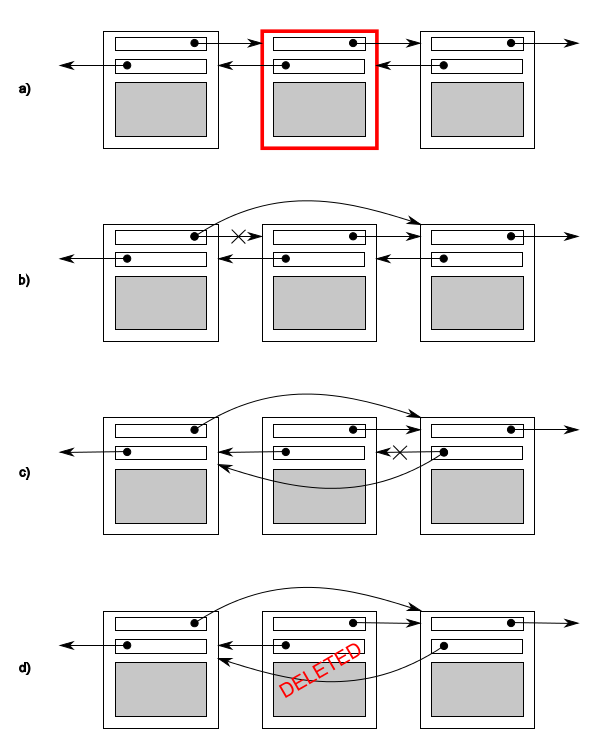
\includegraphics[width=0.7\textwidth]{content/chapter03/images/3-1.png}\\
    图3.1 从一个双链表中删除一个节点
\end{center}


图中b和c在相同方向上的指向和原来已经不一致了,这就破坏了不变量。

线程间的问题在于修改共享数据,会使不变量遭到破坏。删除过程中不确定是否有其他线程能够进行访问,可能就有线程访问到刚刚删除一边的节点。这样破坏了不变量,线程就读取到要删除节点的数据(因为一边的连接被修改,如图3.1(b))。破坏不变量的后果是不确定的,当其他线程按从左到右的顺序访问列表时,将跳过被删除的节点。如有第二个线程尝试删除图中右边的节点,可能会让数据结构产生永久性的损坏,并使程序崩溃。这就是并行中常见错误:条件竞争(race condition)。

\mySubsubsection{3.1.1}{条件竞争}

假如你去一家大电影院买电影票,有很多收银台,很多人可以同时买票。当另一个收银台也在卖你想看电影的电影票时,你的座位选择范围取决于在之前已预定的座位。当只有少量的座位剩下,就可能是一场抢票比赛,看谁能抢到最后一张票。这就是一个条件竞争的例子:你的座位(或者电影票)都取决于购买的顺序。

并发中的竞争条件,取决于一个以上线程的执行顺序,每个线程都抢着完成自己的任务。大多数情况下,即使改变执行顺序,也是良性竞争,结果是可以接受的。例如,两个线程同时向一个处理队列中添加任务,因为不变量保持不变,所以谁先谁后都不会有什么影响。

当不变量遭到破坏时,才会产生条件竞争,比如:双向链表的例子。并发中对数据的条件竞争通常表示为恶性竞争(我们对不产生问题的良性条件竞争不感兴趣)。C++标准中也定义了数据竞争这个术语,一种特殊的条件竞争:并发的去修改一个独立对象(参见5.1.2节),数据竞争是未定义行为的起因。

恶性条件竞争通常发生于对多个数据块的修改,例如:对两个连接指针的修改(如图3.1)。操作要访问两个独立的数据块,独立的指令会对数据块将进行修改,并且其中一个线程可能正在进行修改,另一个线程就对数据块进行了访问。因为出现的概率低,很难查找,也很难复现。如CPU指令连续修改完成后,即使数据结构可以让其他并发线程访问,问题再次复现的几率也相当低。当系统负载增加时,随着执行数量的增加,执行序列问题复现的概率也在增加,这样的问题可能会出现在负载比较大的情况下。条件竞争通常是时间敏感的,所以程序以调试模式运行时,错误常会完全消失,因为调试模式会影响程序的执行时间(即使影响不多)。

当你以写多线程程序为生,条件竞争就会成为你的梦魇。编写软件时,我们会使用大量复杂的操作,来避免恶性条件竞争。

\mySubsubsection{3.1.2}{避免恶性条件竞争}

这里提供一些方法来解决恶性条件竞争,最简单的办法就是对数据结构采用某种保护机制,确保只有修改线程才能看到不变量的中间状态。从其他访问线程的角度来看,修改不是已经完成了,就是还没开始。C++标准库提供很多类似的机制,下面会逐一介绍。

另一个选择是对数据结构和不变量进行修改,修改完的结构必须能完成一系列不可分割的变化,也就保证了每个不变量的状态,这就是所谓的无锁编程。不过,这种方式很难得到正确的结果。到这个级别,无论是内存模型上的细微差异,还是线程访问数据的能力,都会让工作量变的很大。

另一种处理条件竞争的方式,是使用事务的方式去处理数据结构的更新(这里的"处理"就如同对数据库进行更新一样)。所需的一些数据和读取都存储在事务日志中,然后将之前的操作进行合并,再进行提交。当数据结构被另一个线程修改后,或处理已经重启的情况下,提交就会无法进行,这称作为“软件事务内存”(software transactional memory (STM)),这是一个很热门的理论研究领域。这个概念将不会在本书中再进行介绍,因为在C++中没有对STM进行直接支持(尽管C++有事务性内存扩展的技术规范\footnote[1]{SO/IEC TS 19841:2015—Technical Specification for C++ Extensions for Transactional Memory \url{http://www.iso.org/iso/home/store/catalogue_tc/catalogue_detail.htm?csnumber=66343 .}})。

保护共享数据结构的最基本的方式,使用C++标准库提供的互斥量。

% -----

% [1] SO/IEC TS 19841:2015—Technical Specification for C++ Extensions for Transactional Memory http://www.iso.org/iso/home/store/catalogue_tc/catalogue_detail.htm?csnumber=66343 .